\chapter{Pipelines}\label{chapter: pipelines}

\begin{enumerate}
  \item \textbf{Vertex}: The majority of transformation pipeline happens here,
  \textbf{except W2V}
  \begin{itemize}
    \item Programmable through shader
    \item Produces vertices in \textbf{clip space} (a arbitrary region defined
    by graphics APIs in which triangles are drawn)
  \end{itemize}

  \item \textbf{Rasterisation}: produces a set of fragments (which are
  potential pixels); fragments have
  \begin{itemize}
    \item Location in frame buffer (screen location)
    \item Color
    \item Depth
  \end{itemize}

  \item \textbf{Fragment}: the fragment shader would finalize the color
  produced by the rasterisation stage
  \begin{itemize}
    \item Not pixels: each fragment has a 2D location in a raster and a color;
    final value is found by applying hidden surface removal and possibly
    compositing to a set of fragments
    \item Programmable through shader
  \end{itemize}
\end{enumerate}

\section{Transformation Pipeline}

  \begin{equation}
    \begin{bmatrix}
      x_{s} \\
      y_{s} \\
      0 \\
      1
    \end{bmatrix}
    =
    \begin{bmatrix}
      \text{W2V}
    \end{bmatrix}
    \begin{bmatrix}
      \text{Clipping}
    \end{bmatrix}
    \begin{bmatrix}
      \text{Projection}
    \end{bmatrix}
    \begin{bmatrix}
      \text{View}
    \end{bmatrix}
    \begin{bmatrix}
      \text{Model}
    \end{bmatrix}
    \begin{bmatrix}
      x_{m} \\
      y_{m} \\
      z_{m} \\
      1
    \end{bmatrix}
  \end{equation}

  Transforming model coordinate system to viewport coordinate system
  (\textbf{note that transformations occur from right to left})

  \begin{itemize}
    \item Mostly done on GPU (except \textbf{W2V})
    \item GPU parts are done through the vertex shader
    \item Can also handle colors
  \end{itemize}

  \paragraph{Stages}
  \begin{itemize}
    \item The \textbf{model matrix} map local object coordinates to
    world coordinates (ex. rotation)
    \item Given a camera looking down the z-axis from the origin,
    the \textbf{view matrix} map world coordinates to camera coordinates,
    where camera sits at the origin
    \begin{itemize}
      \item Gives us a view volume that is not a cube
    \end{itemize}

    \item The \textbf{projection matrix} map camera coordinates to canonical
    view volume (basically 2D)
    \begin{itemize}
      \item Gives us a clip volume that is a cube
      \item Graphics API typically performs orthographic projection out of
      the box, but \textbf{depth information is preserved} for hidden surface
      removal
      \begin{itemize}
        \item Everything is projected onto $ z = 0 $
      \end{itemize}
    \end{itemize}

    \item \textbf{Clipping}: only contents within the view volume needs to be
    drawn
    \item The \textbf{W2V (window to view) matrix} map canonical view volume
    to screen space; steps
    \begin{enumerate}
      \item \textbf{Clipping}: only draw stuff in clip space
      \item \textbf{Homogeneous divide}
      \item \textbf{Window to view port}: transform from clip coordinates
      (aka. window coordinates $ -1 \to 1 $) to viewport space
    \end{enumerate}
  \end{itemize}

  \textbf{Every transformations except W2V transformation happen in vertex
  processing stage}

  \subsection{In Unity}

    \begin{itemize}
      \item Transform component on a camera is the view matrix
      \item Camera settings are used to create
      \begin{itemize}
        \item Projection matrix
        \item Viewport matrix
      \end{itemize}
    \end{itemize}

\section{Stage - View}

  View transformations translate and rotate all objects in the scene in such
  a way that \textbf{the view of the camera would appear offset and rotated but
  in face at origin (we can't rotate the viewport)}

  \paragraph{Input}
  \begin{itemize}
    \item $ \vec{eye} $: eye position
    \item $ \vec{at} $: look at position
    \item $ \vec{up} $: up vector
  \end{itemize}

  \paragraph{Output}
  \subparagraph{Deriving X, Y, Z Axis}
  \begin{align}
    \vec{v} &= \vec{z} = \vec{at} - \vec{eye} \\
    \vec{n} &= \vec{x} = \vec{z} \times \vec{up} \\
    \vec{u} &= \vec{y} = \vec{x} \times \vec{z}
  \end{align}

  \subparagraph{Deriving Transformation Matrix}
  $ M $ would place the camera on its intended transform. However, since
  we can't transform the camera, we must move everything in the scene instead
  with $ M^{-1} $.

  Left-handed:

  \begin{align}
    M &= T R \\
    M^{-1} &= \left( T R \right)^{-1} \\
    &= R^{-1} T^{-1} \\
    &=
    \begin{bmatrix}
      \vec{n}_{x} & \vec{u}_{x} & \vec{v}_{x} & 0 \\
      \vec{n}_{y} & \vec{u}_{y} & \vec{v}_{y} & 0 \\
      \vec{n}_{z} & \vec{u}_{z} & \vec{v}_{z} & 0 \\
      0 & 0 & 0 & 1
    \end{bmatrix}^{-1}
    \begin{bmatrix}
      1 & 0 & 0 & \vec{eye}_{x} \\
      0 & 1 & 0 & \vec{eye}_{y} \\
      0 & 0 & 1 & \vec{eye}_{z} \\
      0 & 0 & 0 & 1
    \end{bmatrix}^{-1} \\
    &=
    \begin{bmatrix}
      \vec{n}_{x} & \vec{n}_{y} & \vec{n}_{z} & 0 \\
      \vec{u}_{x} & \vec{u}_{y} & \vec{u}_{z} & 0 \\
      \vec{v}_{x} & \vec{v}_{y} & \vec{v}_{z} & 0 \\
      0 & 0 & 0 & 1
    \end{bmatrix}
    \begin{bmatrix}
      1 & 0 & 0 & -\vec{eye}_{x} \\
      0 & 1 & 0 & -\vec{eye}_{y} \\
      0 & 0 & 1 & -\vec{eye}_{z} \\
      0 & 0 & 0 & 1
    \end{bmatrix} \\
    &=
    \begin{bmatrix}
      \vec{n}_{x} & \vec{n}_{y} & \vec{n}_{z} & -\left( \vec{n} \cdot \vec{eye} \right) \\
      \vec{u}_{x} & \vec{u}_{y} & \vec{u}_{z} & -\left( \vec{u} \cdot \vec{eye} \right) \\
      \vec{v}_{x} & \vec{v}_{y} & \vec{v}_{z} & -\left( \vec{v} \cdot \vec{eye} \right) \\
      0 & 0 & 0 & 1
    \end{bmatrix}
  \end{align}

  Right-handed:

  \begin{align}
    M^{-1} =
    \begin{bmatrix}
      \vec{n}_{x} & \vec{n}_{y} & \vec{n}_{z} & \left( \vec{n} \cdot \vec{eye} \right) \\
      \vec{u}_{x} & \vec{u}_{y} & \vec{u}_{z} & \left( \vec{u} \cdot \vec{eye} \right) \\
      \vec{v}_{x} & \vec{v}_{y} & \vec{v}_{z} & \left( \vec{v} \cdot \vec{eye} \right) \\
      0 & 0 & 0 & 1
    \end{bmatrix}
  \end{align}

\section{Stage - Projection}

  Projection refers to the process of reducing dimensionality. There are two
  modes of projection

  \begin{itemize}
    \item \textbf{Ortho}: transform view volume
    \begin{itemize}
      \item The orthograhpic matrix only zero-out the z-axis; the ortho matrix
      transform view volume;
      \item Does not actually perform any projection
      \item The actual orthograhpic projection is left for grahpics APIs
    \end{itemize}

    \item \textbf{Perspective}: scale decreases as distance increases
    \item At this stage, everything is already in the context of the camera;
    the view coordinates
    \item \textbf{Foreshortening}: an illusion that cause an object or distance
    to appear shorter than it actually is
    \begin{itemize}
      \item Occur in both orthographic and perspective projection
    \end{itemize}
  \end{itemize}

  \subsection{Ortho Projection}

    \paragraph{Matrix}
    \begin{align}
      P_{orthographic} &=
      \begin{bmatrix}
        1 & 0 & 0 & 0 \\
        0 & 1 & 0 & 0 \\
        0 & 0 & 0 & 0 \\
        0 & 0 & 0 & 1
      \end{bmatrix} \\
      P_{ortho} &=
      \begin{bmatrix}
        \frac{2}{r - l} & 0 & 0 & -\frac{r + l}{r - l} \\
        0 & \frac{2}{t - b} & 0 & -\frac{t + b}{t - b} \\
        0 & 0 & \frac{-2}{f - n} & -\frac{f + n}{f - n} \\
        0 & 0 & 0 & 1 \\
      \end{bmatrix}
    \end{align}

    This is a combination of a translation (\say{near} might not be at 0)
    and scale matrix

    \begin{itemize}
      \item $ r $: right
      \item $ l $: left
      \item $ t $: top
      \item $ b $: bottom
      \item $ f $: far
      \item $ n $: near
      \item Some WebGL libraries assumes right-handed system cooridnates as
      inputs, despite itself being left-handed, so its ortho matrix also
      inverses the coordinates along z-axis
    \end{itemize}

  \subsection{Perspective Projection}

    \subsubsection{Equation}

      \begin{figure}[H]
        \centering
        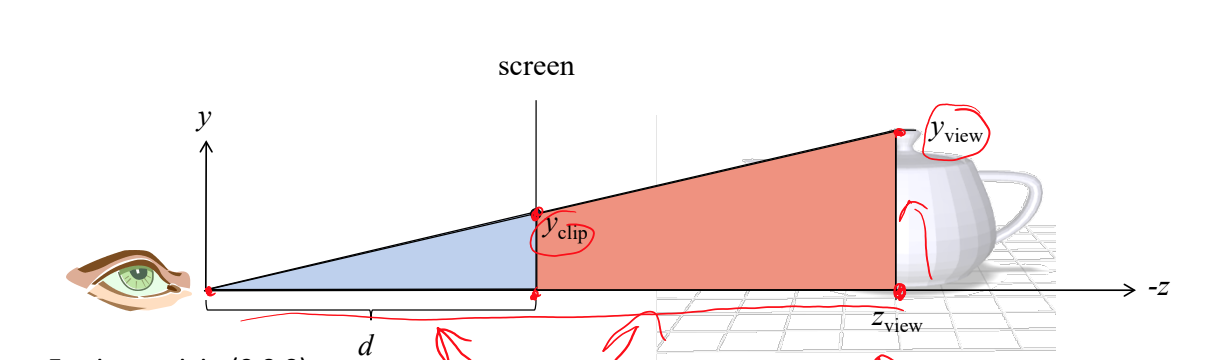
\includegraphics[width=0.7\columnwidth]{images/pipelines/perspective-equation.png}
      \end{figure}

      \begin{align}
        \frac{y_{\text{clip}}}{d}
        &= \frac{y_{\text{view}}}{-z_{\text{view}}} \\
        y_{\text{clip}}
        &= d\frac{y_ {\text{view}}}{-z_{\text{view}}} \\
        &= \frac{y_{\text{view}}}{\frac{-z_{\text{view}}}{d}} \\
        \frac{x_{\text{clip}}}{d}
        &= \frac{x_{\text{view}}}{\frac{-z_{\text{view}}}{d}} \\
        z &= -d
      \end{align}

      \begin{itemize}
        \item The equation applies in situations where
        \begin{itemize}
          \item The \textbf{eyes} are \textbf{centered at the origin}
          \item The \textbf{view} is in \textbf{negative z direction}
          \item The clip is between the eyes and the view
        \end{itemize}

        \item $ d $: distance from eyes to the screen (clip)
        \begin{itemize}
          \item Increasing $ d $; would reduce the size of the image; changing
          $ d $ distort the image
        \end{itemize}
        \item This equation also applies to $ x $ and $ y $
        \item Not invertible
        \item Not an affine transformation (does not preserve the ratio of
        distances)
      \end{itemize}

    \subsubsection{Matrix}

      The perspective projection matrix also needs to do what the ortho matrix
      does, scaling coordinates so that everything fits inside the clip space

      \begin{equation}
        P =
        \begin{bmatrix}
          \frac{n}{r} & 0 & 0 & 0 \\
          0 & \frac{n}{t} & 0 & 0 \\
          0 & 0 & \frac{-f}{f - n} & \frac{-fn}{f - n} \\
          0 & 0 & -1 & 0 \\
        \end{bmatrix}
      \end{equation}

      \begin{itemize}
        \item $ r $: right
        \item $ t $: top
        \item $ n $: near
        \item $ f $: far
        \item This gives the frustum matrix, which is asymmetrical
        perspective matrix is symmetrical
      \end{itemize}

      \href{http://www.songho.ca/opengl/gl_projectionmatrix.html}{Deriving
      the matrix}

\section{Stage - Window to Viewport}

  This is the transformation used by systems where the
  $ x \in \left[ -1, 1 \right], y \in \left[ -1, 1 \right] $; in essence,
  the matrix (from right to left)

  \begin{enumerate}
    \item Translate the lower left corner to $ \left( 0, 0 \right) $
    \item Scale the upper right corner to $ \left( w - 1, h - 1 \right) $
  \end{enumerate}

  \begin{align}
    \text{W2V } &=
    \begin{bmatrix}
      \frac{w - 1}{2} & 0 & 0 \\
      0 & \frac{h - 1}{2} & 0 \\
      0 & 0 & 1
    \end{bmatrix}
    \begin{bmatrix}
      1 & 0 & 1 \\
      0 & 1 & 1 \\
      0 & 0 & 1
    \end{bmatrix}
    \begin{bmatrix}
      x \\
      y \\
      1
    \end{bmatrix} \\
    &=
    \begin{bmatrix}
      \frac{w - 1}{2} & 0 & \frac{w - 1}{2} \\
      0 & \frac{h - 1}{2} & \frac{h - 1}{2} \\
      0 & 0 & 1
    \end{bmatrix}
    \begin{bmatrix}
      x \\
      y \\
      1
    \end{bmatrix}
  \end{align}

  \begin{itemize}
    \item $ w $: viewport width
    \item $ h $: viewport height
  \end{itemize}

  \subsection{Continuous Space}

    Even though pixels are discrete units (you can't have half of a pixel),
    it can be helpful to still consider pixel spaces to be continuous; WebGL
    and DirectX considers pixel centers to be
    $ \left( x + 0.5, y + 0.5 \right) $

\section{Hidden Surface Removal}

  \begin{itemize}
    \item \textbf{Painter's algorithm}: draw farther object first
    \begin{itemize}
      \item Expensive to sort
      \item Depth cycle
    \end{itemize}

    \item \textbf{Z-Buffer}: keep a z buffer on pixels, while drawing,
    only write to pixel if the object being drawn has a z value that is
    closer than the z value of the pixel
    \begin{itemize}
      \item More popular today; not used in the past for memory issues
      \item If two z values are too close, it's hard to determine which is
      closer
    \end{itemize}

    \item \textbf{Aka. depth test}
  \end{itemize}
